\documentclass[../cnd.tex]{subfiles}

Đây là một ứng dụng rất đơn giản để giới thiệu về một trong các ứng dụng quan trọng của nền tảng Ethereum - ứng dụng phi tập trung (decenterlized app). Mọi dữ liệu đều bị ẩn danh và không thể sửa đổi nhưng có một khuyết điểm là để sử dụng nó, người dùng cần cài đặt một chương trình để có thể tham gia vào mạng Ethereum, điều này khá khó và phức tạp cho một người dùng cuối. Vì vậy mà đã có rất nhiều ứng dụng hướng việc sử dụng các ứng dụng phi tập trung như một ứng dụng web thông thường, ví dụ như \url{kyber.network}. 

Ứng dụng đơn giản này được viết ra để mô phỏng lại việc đó cũng như hướng dẫn bạn có thể làm được một ứng dụng như thế. Ứng dụng mô tả một cuộc bầu cử đơn giản, những đặc tính của ứng dụng phi tập trung khá phù hợp cho công việc này - ẩn danh và không thể thay đổi.

\subsection{Mô tả ứng dụng}
Ứng dụng cho phép người dùng thông thường đăng ký một tài khoản Ethereum mới hoặc nhập lại tài khoản đã có sẵn trên mạng thử nghiệm (ứng dụng này sử dụng mạng thử nghiệm của Ethereum có tên là Rinkeby$^{[10]}$) mà không cần cài đặt thêm chương trình ngoài, có thể dùng nó như một ứng dụng web.

Trước tiên nên nói về lí do chọn mạng thử nghiệm Rinkeby mà không phải mạng khác (Ethereum còn hai mạng thử nghiệm khác là Ropsten$^{[11]}$ và Kovan$^{[12]}$ tính đến thời điểm viết bài viết này). Lí do đầu tiên chắc chắn là từ sự đơn giản trong việc cài đặt với chỉ một vài dòng lệnh trên Linux, thứ hai là đây là mạng trẻ nhất nên số khối cũng ít nhất do đó chúng ta sẽ không phải đồng bộ quá nhiều khối. Bên cạnh đó, việc chúng ta có thể xin ether miễn phí khá đơn giản và thuận tiện. 

Những lí do được nêu ra ở trên khá là chủ quan và thiên về việc phát triển ứng dụng, lí do khách quan để mạng thử ngiệm thứ ba được ra đời bắt nguồn từ các yếu điểm của hai mạng thử nghiệm trước đó. Mạng Ropsten hoạt động rất tốt trong thời gian đầu nhưng vì hàm băm dùng cho quá trình đào ở mạng này khá yếu (để các máy tính cá nhân có thể đào được) nên dễ dàng bị những kẻ phá hoại tấn công spam, từ đó mạng Kovan ra đời khắc phục hoàn toàn điểm yếu đó - không còn việc đào ether nữa và các giao dịch được các bên tin cậy xác nhận. Mạng Kovan này hoạt động rất hiệu quả nhưng lại nảy sinh vấn đề với Parity (chương trình cần cài đặt để tham gia mạng này), chỉ những người dùng Parity mới có thể tham gia vào mạng này mà không thể dùng chương tình tùy chọn khác và lí do đó đã thúc đẩy Rikeby ra đời hỗ trợ người dùng có thể dùng các chương trình khác nhau để kết nối với mạng. Vì những ưu thế đó, chúng ta sẽ sử dụng mạng thử nghiệm Rinkeby.

Để có thể bầu chọn trong ứng dụng, người sử dụng sẽ cần có ether trong tài khoản bằng cách xin cấp miễn phí tại \url{https://faucet.rinkeby.io}. Khi đã có ether trong tài khoản của mình, người dùng có thể sử dụng chức năng bầu cử và chỉ được bầu cử một lần duy nhất với mỗi tài khoản Ethereum. 

Do sử dụng mạng thử nghiệm nên tốc độ phản hồi khá là chậm nên có thể gây phiền toái đôi chút nhưng đủ với một ứng dụng thử nghiệm.

\subsection{Yêu cầu chính của ứng dụng}
\begin{itemize}
\item Phiên bản nodejs $\geq$ 6.0.0
\item Phiên bản npm $\leq$ 3.0.0
\item Phiên bản geth $\geq$ 1.7.0
\end{itemize}

\subsection{Tạo lập môi trường giao tiếp với mạng Ethereum}

Phần hướng dẫn sau đây là dành cho môi trường phát triển trên Linux (cụ thể hơn là Ubuntu), các môi trường khác có thể thực hiện theo các bước tương tự với một số thay đổi. Để có thể triển khai ứng dụng, cần có một chương trình chạy trên máy chủ giao tiếp với mạng thử nghiệm Rinkeby có tên là Go Ethereum (Geth). 

Để cài đặt ta thực hiện:
\lstset{
	basicstyle=\footnotesize,
	xleftmargin=.1\textwidth, xrightmargin=.2\textwidth
}
\begin{lstlisting}[language=bash]
sudo add-apt-repository -y ppa:ethereum/ethereum
sudo apt-get update
sudo apt-get install ethereum
\end{lstlisting}


Sau khi cài đặt xong để chạy Geth ta sẽ dùng câu lệnh:
\begin{lstlisting}[language=bash]
geth --rinkeby --rpc --rpcapi db,eth,net,web3,personal
\end{lstlisting}

Ta sẽ thấy một số tham số, --rinkeby để chỉ định mạng thử nghiệm mà chúng ta sử dụng, --rpcapi chỉ định các giao diện lập trình ứng dụng mà ta có thể sử dụng để giao tiếp với chương trình Geth này. Sau khi thực hiện câu lệnh, bạn sẽ phải đợi một khoảng thời gian đáng kể để chương trình tải về chuỗi khối, bạn phải lưu ý rằng chương trình phải có chuỗi khối mới nhất thì mới có thể thực hiện giao dịch nhưng vẫn có thể nhận ether một cách bình thường hay nói cách khác là có thể nhận giao dịch vào mà không thể thực hiện giao dịch ra. 

Bạn cũng có thể dùng luôn bản điều khiển của Geth để kết nối và thực hiện một vài yêu cầu như tạo tài khoản, lấy số dư bằng câu lệnh:
\begin{lstlisting}[language=bash]
geth --datadir=$HOME/.rinkeby attach ipc:$HOME/.rinkeby/geth.ipc console
\end{lstlisting}

Vậy là ta đã có một nút trên mạng Ethereum và có thể sử dụng web3$^{[13]}$ - một thư viện cung cấp các giao diện lập trình trên mạng Ethereum để thực hiện các yêu cầu theo mong muốn của ứng dụng bầu cử. Việc sử dụng thư viện trên nhằm mục đích giúp ứng dụng web có thể sử dụng các câu lệnh được hỗ trợ trên nút ethereum thông qua một giao diện mà ứng dụng có thể sử dụng được.

\subsection{Xây dựng ứng dụng}

Sau khi đã thiết lập nút Ethereum và thư viện giao tiếp, ta sẽ tiếp tục với việc xây dựng phần chính (nội dung) cho ứng dụng. 

Chúng ta sẽ phải xây dựng ứng dụng với ba phần: phần hơp đồng thông minh, phần backend và phần frontend. Những ngôn ngữ ta cần sử dụng là Solidity cho phần hợp đồng thông minh và JavaScript cho phần backend và frontend. Phía backend sẽ sử dụng nodejs nên trước khi tiếp tục bạn cần cài đặt nodejs, quá trình cài đặt khá đơn giản và bạn hoàn toàn có thể tự hoàn thành được.

\subsubsection{Hợp đồng thông minh}
Hợp đồng thông minh của ứng dụng bầu cử này sẽ được viết bằng ngôn ngữ Solidity. Vì chương trình đơn giản nên hợp đồng sẽ khá ngắn, cú pháp của Solidity khá giống với JavaScript nên tương đối dễ hiểu. 

Sau khi hoàn thành mã nguồn của hợp đồng thông minh, ta sẽ cần biên dịch mã nguồn đó trước khi có thể triển khai trên máy ảo Ethereum, mỗi lần thay đổi mã nguồn bạn sẽ phải làm lặp lại các bước trên khá là phức tạp và phiền toái, nên ứng dụng này sẽ sử dụng khung làm việc Truffle$^{[14]}$ để hoàn thành các công việc trên một cách tự động.

Một số điều cần lưu ý khi triển khai hợp đồng trên máy ảo Ethereum là bạn cần một tài khoản và ether để triển khai hợp đồng. Để thực hiện các giao dịch cũng như chi tiêu đồng ether này, bạn phải mở khóa tài khoản đó bằng cách chạy lại Geth và thêm tham số --unlock= cộng với giá trị theo sau là địa chỉ tài khoản của bạn. Ví dụ --unlock="0x176916e03344eef8B7c85e18D488d71437966333". 

Sau đó chương trình sẽ yêu cầu bạn nhập mật khẩu để xác nhận bạn sở hữu tài khoản đó. Tiếp theo ta cần chỉnh sửa tệp truffle.js như sau:

\begin{lstlisting}[language=c]
module.exports = {
  networks: {
    rinkeby: {
      host: "localhost", // Connect to geth on the specified
      port: 8545,
      from: "0x176916e03344eef8B7c85e18D488d71437966333",
      network_id: 4,
      gas: 4000000 // Gas limit used for deploys
    }
  }
};
\end{lstlisting}

Như chúng ta thấy file này sẽ chứa:
\begin{itemize}
	\item host: địa chỉ ip của nút Ethereum
	\item port: cổng của nút Ethereum
	\item from: địa chỉ sẽ chi ether để triển khai	
	\item network_id: chỉ định mạng sẽ được triển khai (id của mạng Rinkeby là 4)	
	\item gas: chỉ mức bạn chi để triển khai hợp đồng (nếu quá nhỏ sẽ không thể triển khai)
\end{itemize}

Sau khi triển khai xong ta sẽ có tệp Voting.json, tệp này sẽ được chứa các cấu hình để có thể gọi các phương thức của hợp đồng. Cấu trúc của tệp json khá đơn giản gồm mã nguồn đã biên dịch của hợp đồng, địa chỉ hợp đồng trên mạng và một số trường khác.

\subsubsection{Backend}
Phía backend sẽ được viết bằng nodejs để đảm bảo tương thích tốt nhất với web3 (đã có các bản phân phối cho các ngôn ngữ khác). Phiên bản web3 sử dụng trong ứng dụng này là phiên bản beta nhưng có nhiều tính năng mới và tương thích tôt hơn, tài liệu sử dụng cụ thể tại \url{https://web3js.readthedocs.io/en/1.0}. 

Việc tạo tài khoản khá đơn giản bằng việc gọi một phương thức của web3, ta chỉ cần chú ý rằng kết quả trả về sẽ gồm một khóa công khai (địa chỉ của tài khoản) và một khóa bí mật. Muốn lưu lại khóa bí mật này ta cần mã hóa nó với mật khẩu do người dùng nhập vào, web3 cũng hỗ trợ việc này với phương thức mã hóa AES với độ dài khóa 128 bit. 

Một điều cần lưu ý dù nó đã được mã hóa với độ dài khóa đủ lớn nhưng cũng phải tránh các trường hợp bị lộ thông tin này do mật khẩu của người dùng thường nằm trong tập từ điển nhỏ hơn (để dễ nhớ) nên khả năng bị tấn công vét cạn vẫn có thể xảy ra. Điều đó cũng khuyên bạn rằng không nên để quá nhiều ether vào trong một tài khoản do dùng một khóa càng nhiều lần thì càng gia tăng khả năng bị lộ khóa.

Vì là ứng dụng thử nghiệm nên ta sẽ chỉ đơn giản định danh mỗi người dùng bởi một token (sẽ được tạo tự động trong lần đầu tiên truy cập), và mỗi tài khoản người dùng có thể tạo nhiều tài khoản Ethereum, mỗi tài khoản này sẽ có thể tải về khóa bí mật của họ (đã được mã hóa trước đó) để sử dụng lại về sau. Điều này cũng được áp dụng trong \textit{kyber.network} bản thử nghiệm và ví Mist (thực chất Mist được phát triển như là một trình duyệt cho các ứng dụng phi tập trung) nên cũng không quá tồi nếu ta dùng giải pháp này thay vì bắt người dùng đăng ký một tài khoản để lưu trữ các tài khoản Ethereum khác.

Vấn đề chính cần giải quyết là việc mở khóa tài khoản để có thể sử dụng ether trong quá trình bầu cử (muốn thưc hiện giao dịch ra cần có khóa bí mật để ký). Về mặt tài liệu, web3 đã cung cấp phương thức mở khóa tài khoản bằng địa chỉ và mật khẩu trong một khoảng thời gian nhất định. Nhưng chú ý rằng bạn không thể dùng phương thức đó nếu bạn không thực hiện bước lưu khóa bí mật đã mã hóa tại thư mục \$HOME/.ethereum/rinkeby/keystore. 

Thông thường khi bạn tạo tài khoản, tệp lưu khóa bí mật này sẽ được tạo tự động nhưng nếu tạo với web3 thì không, vì vậy bạn phải tạo thủ công bằng nghiệp vụ bên ứng dụng web mỗi khi có yêu cầu đăng ký tài khoản Ethereum. Hãy để thời gian mở khóa một cách hợp lý để cân bằng giữa tính tiện dụng và bảo mật cho ứng dụng, không nên để quá dài.

Việc cần làm tiếp theo là việc chuyển các yêu cầu của người dùng thành các yêu cầu gửi tới hợp đồng để tác động lên chuỗi khối, chú ý rằng đây là mạng thử nghiệm nên nó khá chậm và sẽ mất một khoảng thời gian đáng kể cho mỗi giao dịch.

Để chạy chương tình phía backend bạn cần vào thư mục chứa mã nguồn của phần này và chạy câu lệnh, ứng dụng sẽ chạy mặc định tại cổng 3333.
\begin{lstlisting}[language=bash]
npm run server:dev
\end{lstlisting}

\subsubsection{Frontend}
Phía frontend được viết bằng khung làm việc VueJS$^{[15]}$, được sử dụng để xây dựng ứng dụng một trang (Single Page Application) một cách nhanh chóng.

Để chạy chương trình phía frontend bạn cần chạy câu lệnh:
\begin{lstlisting}[language=bash]
npm run dev
\end{lstlisting}

Câu lệnh trên chỉ sử dụng khi ở chế độ phát triển và nếu muốn đưa vào triển khai thì bạn phải chạy câu lệnh: 
\begin{lstlisting}[language=bash]
npm run build
\end{lstlisting}
Các tệp html, css, js sẽ được sinh tự động để bạn có thể đưa vào ứng dụng phía backend. Cách trên khá bất tiện nên trong phiên bản tiếp theo sẽ có chỉnh sửa để quá trình được tự động hơn. 

\subsubsection{Hình ảnh từ ứng dụng}

\begin{figure}[H]
\centering
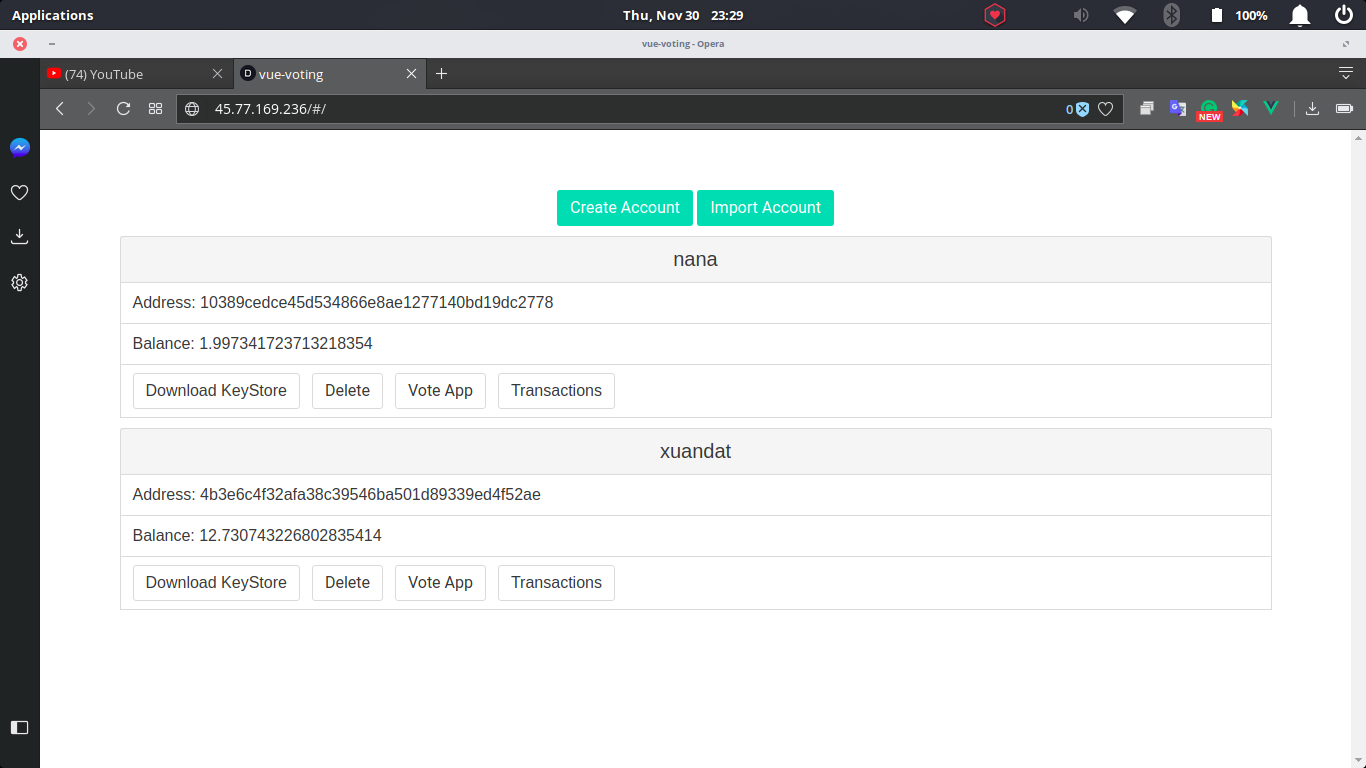
\includegraphics[width=0.85\textwidth]{../img/main}
\caption{Trang chủ ứng dụng}
\end{figure}

\begin{figure}[H]
\centering
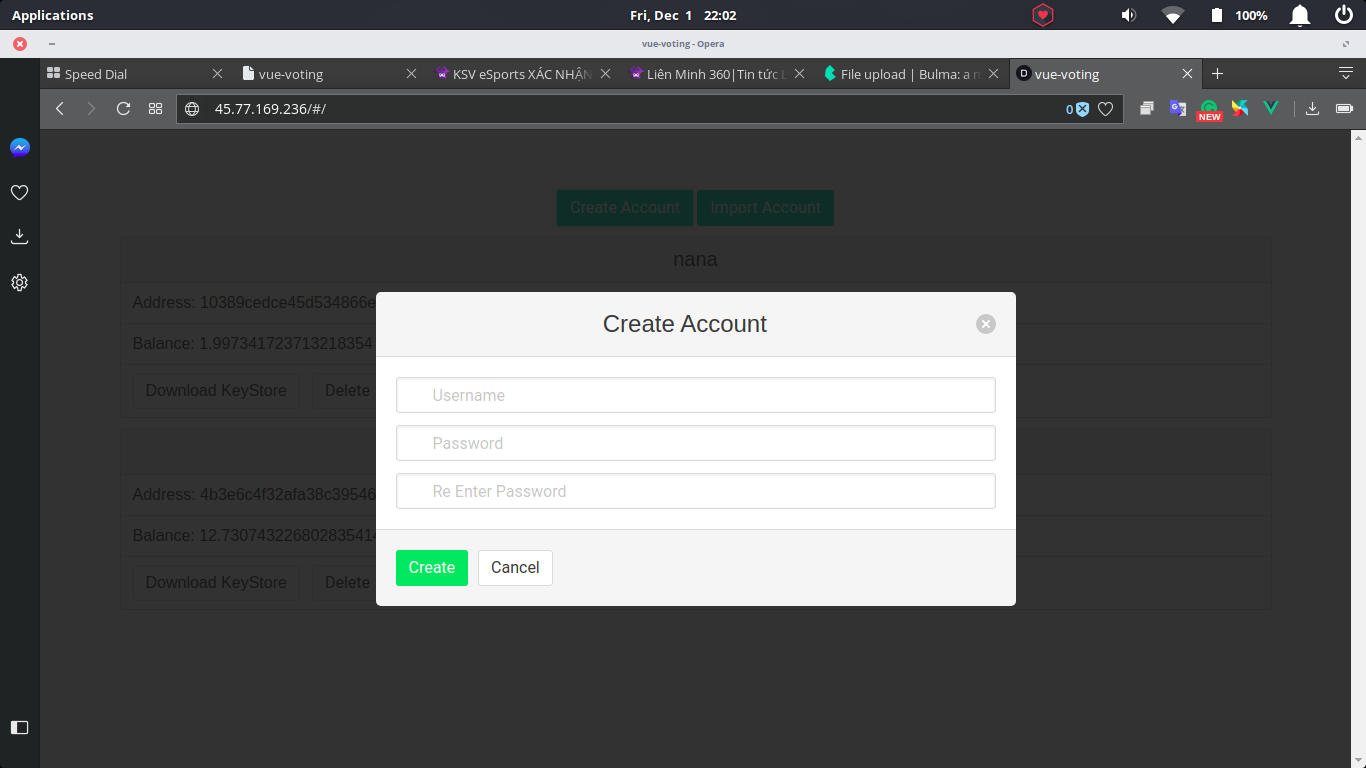
\includegraphics[width=0.85\textwidth]{../img/new}
\caption{Thêm tài khoản}
\end{figure}

\begin{figure}[H]
\centering
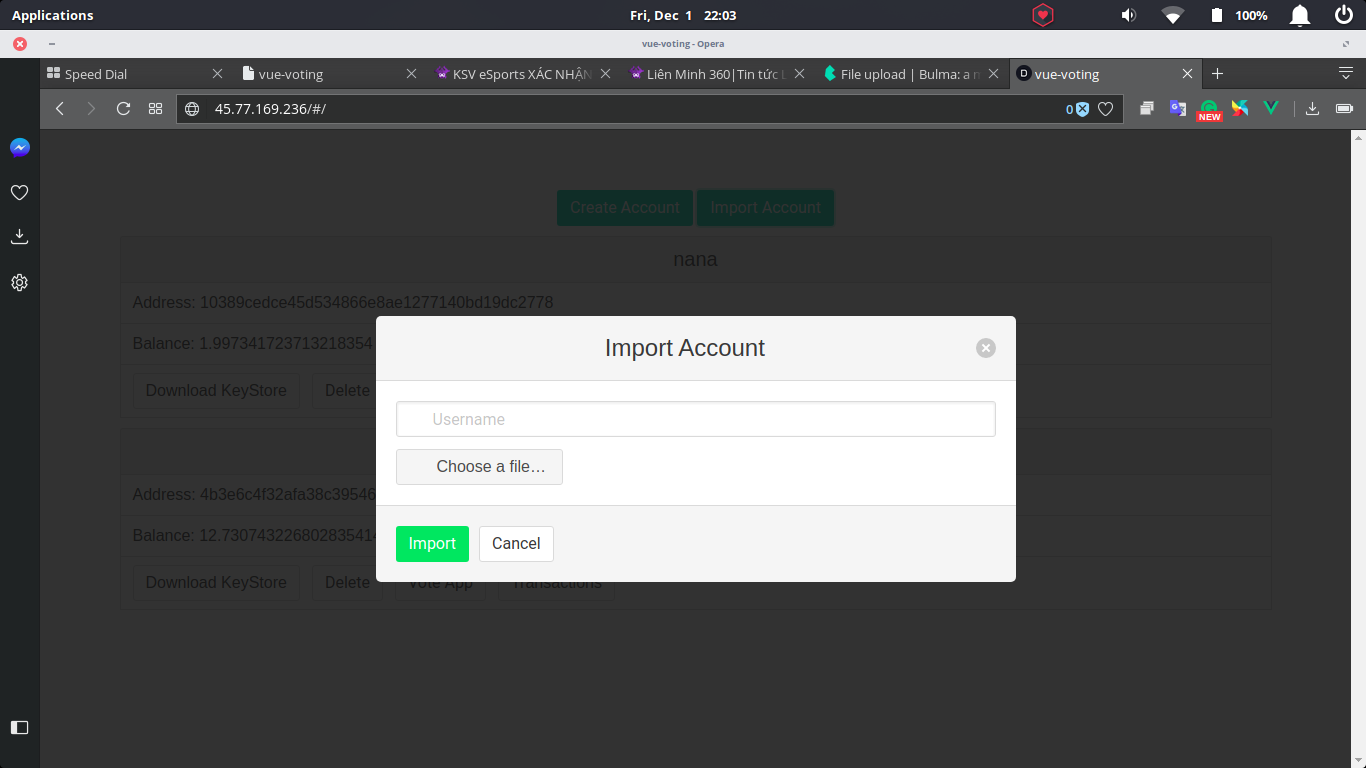
\includegraphics[width=0.85\textwidth]{../img/import}
\caption{Nhập tài khoản}
\end{figure}

\begin{figure}[H]
\centering
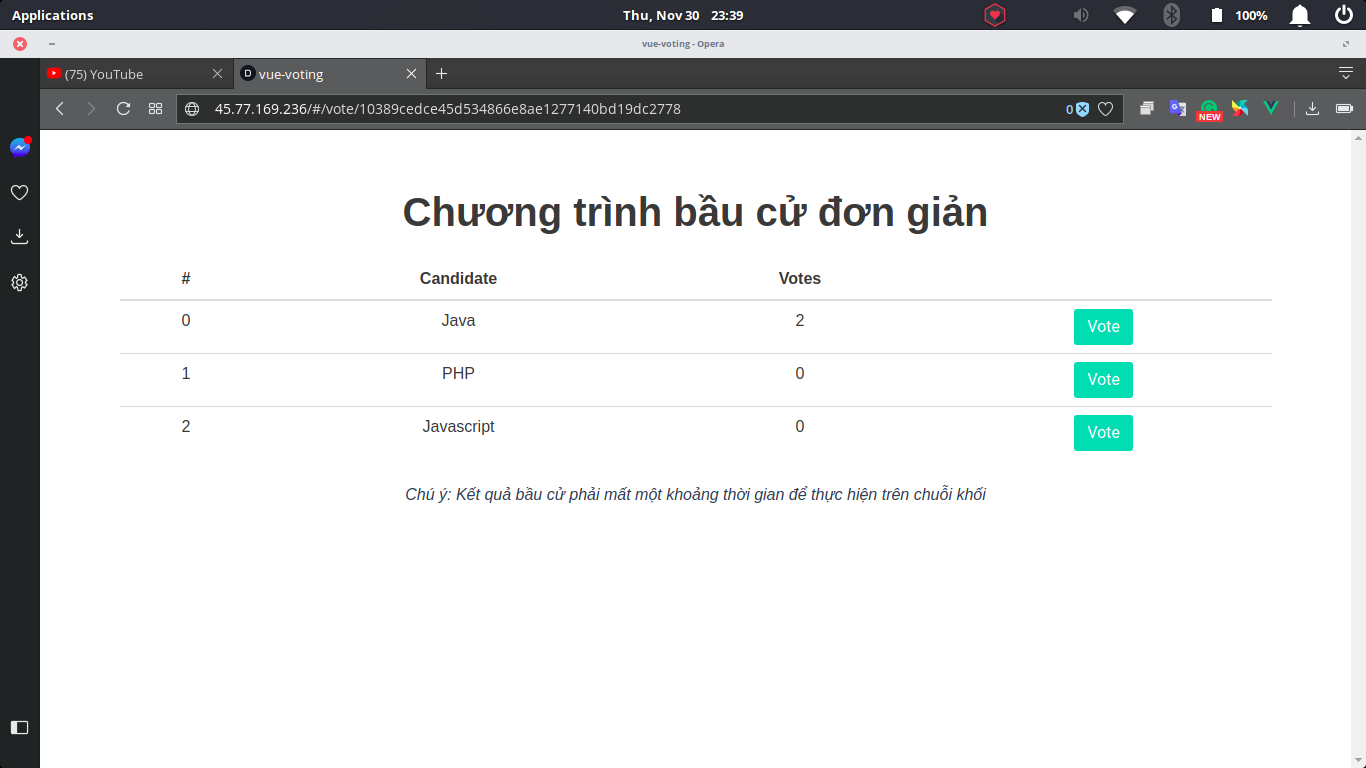
\includegraphics[width=0.85\textwidth]{../img/app}
\caption{Ứng dụng bầu cử}
\end{figure}

\begin{figure}[H]
\centering
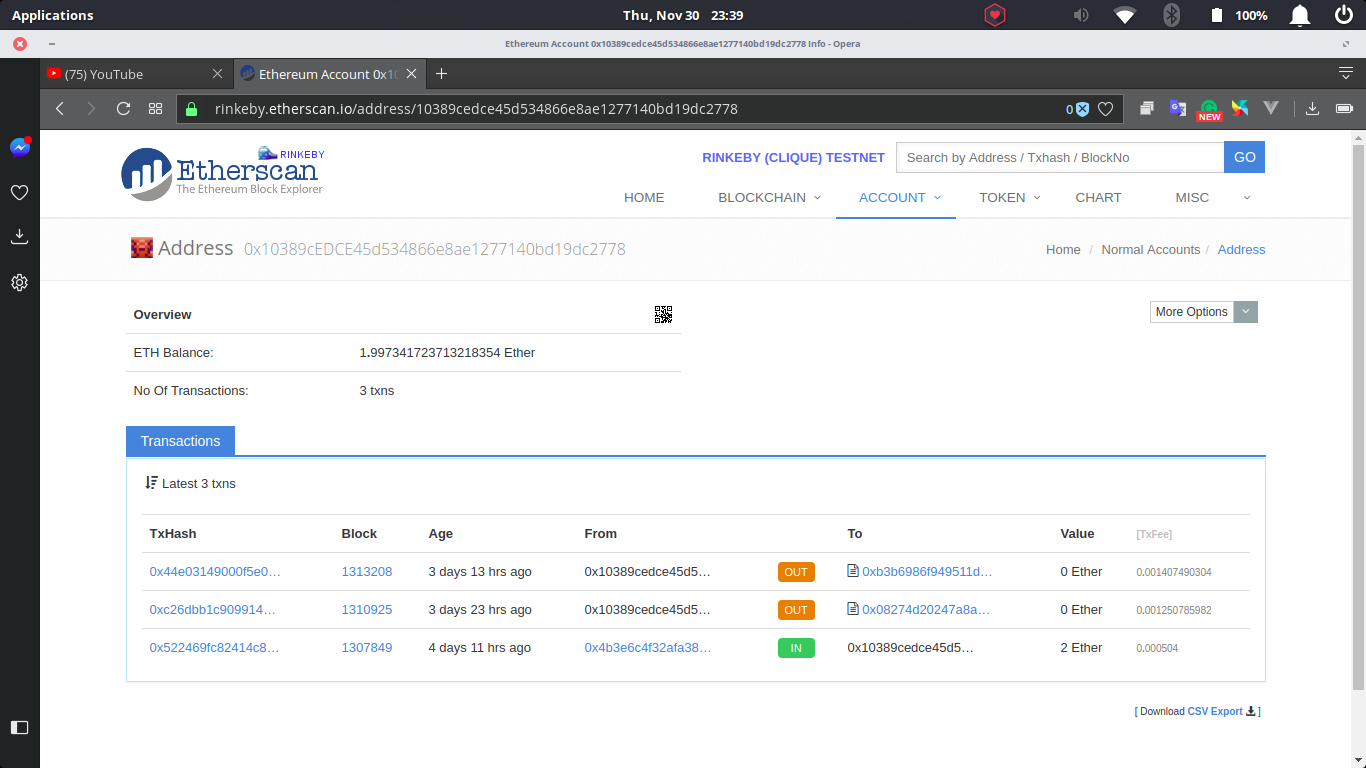
\includegraphics[width=0.85\textwidth]{../img/transaction}
\caption{Trang cung cấp tra cứu giao dịch}
\end{figure}

\subsubsection{Một số lưu ý rút ra từ ứng dụng}
Phần này được viết thêm và sẽ hữu ích với bạn nếu bạn định sử dụng Ethereum trong mạng thật và chi tiêu cũng như đầu tư vào Ethreum. Nếu bạn đọc mã nguồn của chương trình cũng như có thể suy đoán ra, chương trình trên hoàn toàn có thể có được khóa bí mật của bạn và đó là một rủi ro nếu bạn sử dụng đồng ether thật. 

Cụ thể với trang \url{https://www.blockchain.com}, bạn cũng có thể tạo tài khoản một cách trực tuyến mà không phải cài đặt gì, nhận tiền và chuyển tiền và bạn cũng có thể bị mất nó bất kì lúc nào. Bạn dùng nó và chỉ mong nhà cung cấp dịch vụ không làm gì với thông tin cá nhân của mình, cũng như các dịch vụ tập trung khác mà bạn đang sử dụng. Vì vậy nếu muốn an tâm hoàn toàn, bạn nên cài đặt các ví được cung cấp một cách chính thống như \url{https://github.com/ethereum/mist/releases}. Bạn vẫn có nguy cơ bị tấn công nhưng ít nhất bạn biết bạn đang giữ tài sản của mình.